%% LyX 2.3.4.2 created this file.  For more info, see http://www.lyx.org/.
%% Do not edit unless you really know what you are doing.
\documentclass[english,dvipsnames,aspectratio=169,handout]{beamer}
\usepackage{mathptmx}
\usepackage{eulervm}
\usepackage[T1]{fontenc}
\usepackage[latin9]{inputenc}
\usepackage{babel}
\usepackage{amstext}
\usepackage{amssymb}
\usepackage{graphicx}
\usepackage{ifthen}
\usepackage{xcolor}
\usepackage{xspace}
\usepackage{tikz}
\usetikzlibrary{tikzmark}
\usetikzlibrary{calc}
\usepackage{pgfplots}
%\pgfplotsset{compat=1.17}
\usepackage{booktabs}
\usepackage{xpatch}
\usepackage{multirow}
\usepackage{colortbl}
\usepackage{pgfpages}




\xpatchcmd{\itemize}
  {\def\makelabel}
  {\ifnum\@itemdepth=1\relax
     \setlength\itemsep{2ex}% separation for first level
   \else
     \ifnum\@itemdepth=2\relax
       \setlength\itemsep{1ex}% separation for second level
     \else
       \ifnum\@itemdepth=3\relax
         \setlength\itemsep{0.5ex}% separation for third level
   \fi\fi\fi\def\makelabel
  }
 {}
 {}

\ifx\hypersetup\undefined
  \AtBeginDocument{%
    \hypersetup{unicode=true,pdfusetitle,
 bookmarks=true,bookmarksnumbered=false,bookmarksopen=false,
 breaklinks=false,pdfborder={0 0 0},pdfborderstyle={},backref=false,colorlinks=true,
 allcolors=NYUPurple,urlcolor=LightPurple}
  }
\else
  \hypersetup{unicode=true,pdfusetitle,
 bookmarks=true,bookmarksnumbered=false,bookmarksopen=false,
 breaklinks=false,pdfborder={0 0 0},pdfborderstyle={},backref=false,colorlinks=true,
 allcolors=NYUPurple,urlcolor=LightPurple}
\fi

\makeatletter

%%%%%%%%%%%%%%%%%%%%%%%%%%%%%% LyX specific LaTeX commands.
%% Because html converters don't know tabularnewline
\providecommand{\tabularnewline}{\\}

%%%%%%%%%%%%%%%%%%%%%%%%%%%%%% Textclass specific LaTeX commands.
% this default might be overridden by plain title style
\newcommand\makebeamertitle{\frame{\maketitle}}%
% (ERT) argument for the TOC
\AtBeginDocument{%
  \let\origtableofcontents=\tableofcontents
  \def\tableofcontents{\@ifnextchar[{\origtableofcontents}{\gobbletableofcontents}}
  \def\gobbletableofcontents#1{\origtableofcontents}
}

%%%%%%%%%%%%%%%%%%%%%%%%%%%%%% User specified LaTeX commands.
\usetheme{CambridgeUS} 
\beamertemplatenavigationsymbolsempty


% Set Color ==============================
\definecolor{NYUPurple}{RGB}{87,6,140}
\definecolor{LightPurple}{RGB}{165,11,255}


\setbeamercolor{title}{fg=NYUPurple}
\setbeamercolor{frametitle}{fg=NYUPurple}

\setbeamercolor{background canvas}{fg=NYUPurple, bg=white}
\setbeamercolor{background}{fg=black, bg=NYUPurple}

\setbeamercolor{palette primary}{fg=black, bg=gray!30!white}
\setbeamercolor{palette secondary}{fg=black, bg=gray!20!white}
\setbeamercolor{palette tertiary}{fg=gray!20!white, bg=NYUPurple}

\setbeamertemplate{headline}{}
\setbeamerfont{itemize/enumerate body}{}
\setbeamerfont{itemize/enumerate subbody}{size=\normalsize}

\setbeamercolor{parttitle}{fg=NYUPurple}
\setbeamercolor{sectiontitle}{fg=NYUPurple}
\setbeamercolor{sectionname}{fg=NYUPurple}
\setbeamercolor{section page}{fg=NYUPurple}
%\setbeamercolor{description item}{fg=NYUPurple}
%\setbeamercolor{block title}{fg=NYUPurple}

\setbeamertemplate{blocks}[rounded][shadow=false]
\setbeamercolor{block body}{bg=normal text.bg!90!NYUPurple}
\setbeamercolor{block title}{bg=NYUPurple!30, fg=NYUPurple}



\AtBeginSection[]{
  \begin{frame}
  \vfill
  \centering
\setbeamercolor{section title}{fg=NYUPurple}
 \begin{beamercolorbox}[sep=8pt,center,shadow=true,rounded=true]{title}
    \usebeamerfont{title}\usebeamercolor[fg]{title}\insertsectionhead\par%
  \end{beamercolorbox}
  \vfill
  \end{frame}
}

\makeatother

\setlength{\parskip}{\medskipamount} 

\input ../macros

\begin{document}
\input ../rosenberg-macros

%\setbeameroption{show notes on second screen}

\title[DS-GA 1003]{$k$-Means Clustering}
\author{He He \\
Slides based on Lecture
\href{https://github.com/davidrosenberg/mlcourse/blob/gh-pages/Lectures/13a.k-means.pdf}{13a} from David Rosenberg's course materials (\url{https://github.com/davidrosenberg/mlcourse})
}
\date{April 27, 2021}
\institute{CDS, NYU}

\makebeamertitle
\mode<article>{Just in article version}

\begin{frame}
{Unsupervised learning}
\begin{description}[<+->]
\item[Goal] Discover interesting \emph{structure} in the data.
\item[Formulation] Density estimation: $p(x;\theta)$ (often with \emph{latent} variables).
\item[Examples]
\begin{itemize}[<.->]
\item Discover \emph{clusters}: cluster data into groups.
\item Discover \emph{factors}: project high-dimensional data to a small number of ``meaningful'' dimensions, \ie dimensionality reduction.
\item Discover \emph{graph structures}: learn joint distribution of correlated variables, \ie graphical models.
\end{itemize}
\end{description}
\note[item]{Most of what we have learned so far belongs to supervised learning, where the core problem is to make predictions on unseen data given labeled training data. There is another important type of ML called unsupervised learning, where the main goal is to discover interesting patterns in the data.}
\note[item]{Unlike supervised learning, there is no obvious loss function since we don't know what patterns to look for. Instead, the problem is often formulated as density estimation where we aim to maximize the likelihood of the observed data.}
\note[item]{Clusters: group documents into different topics.}
\note[item]{Factors: variation among face images can be explained by a few factors such as illumination, pose, identity etc.}
\note[item]{Graph: phylogenetic tree of DNA evolution.}
\note[item]{We'll focus on clustering today.}
\end{frame}

\begin{frame}{Example: Old Faithful Geyser}
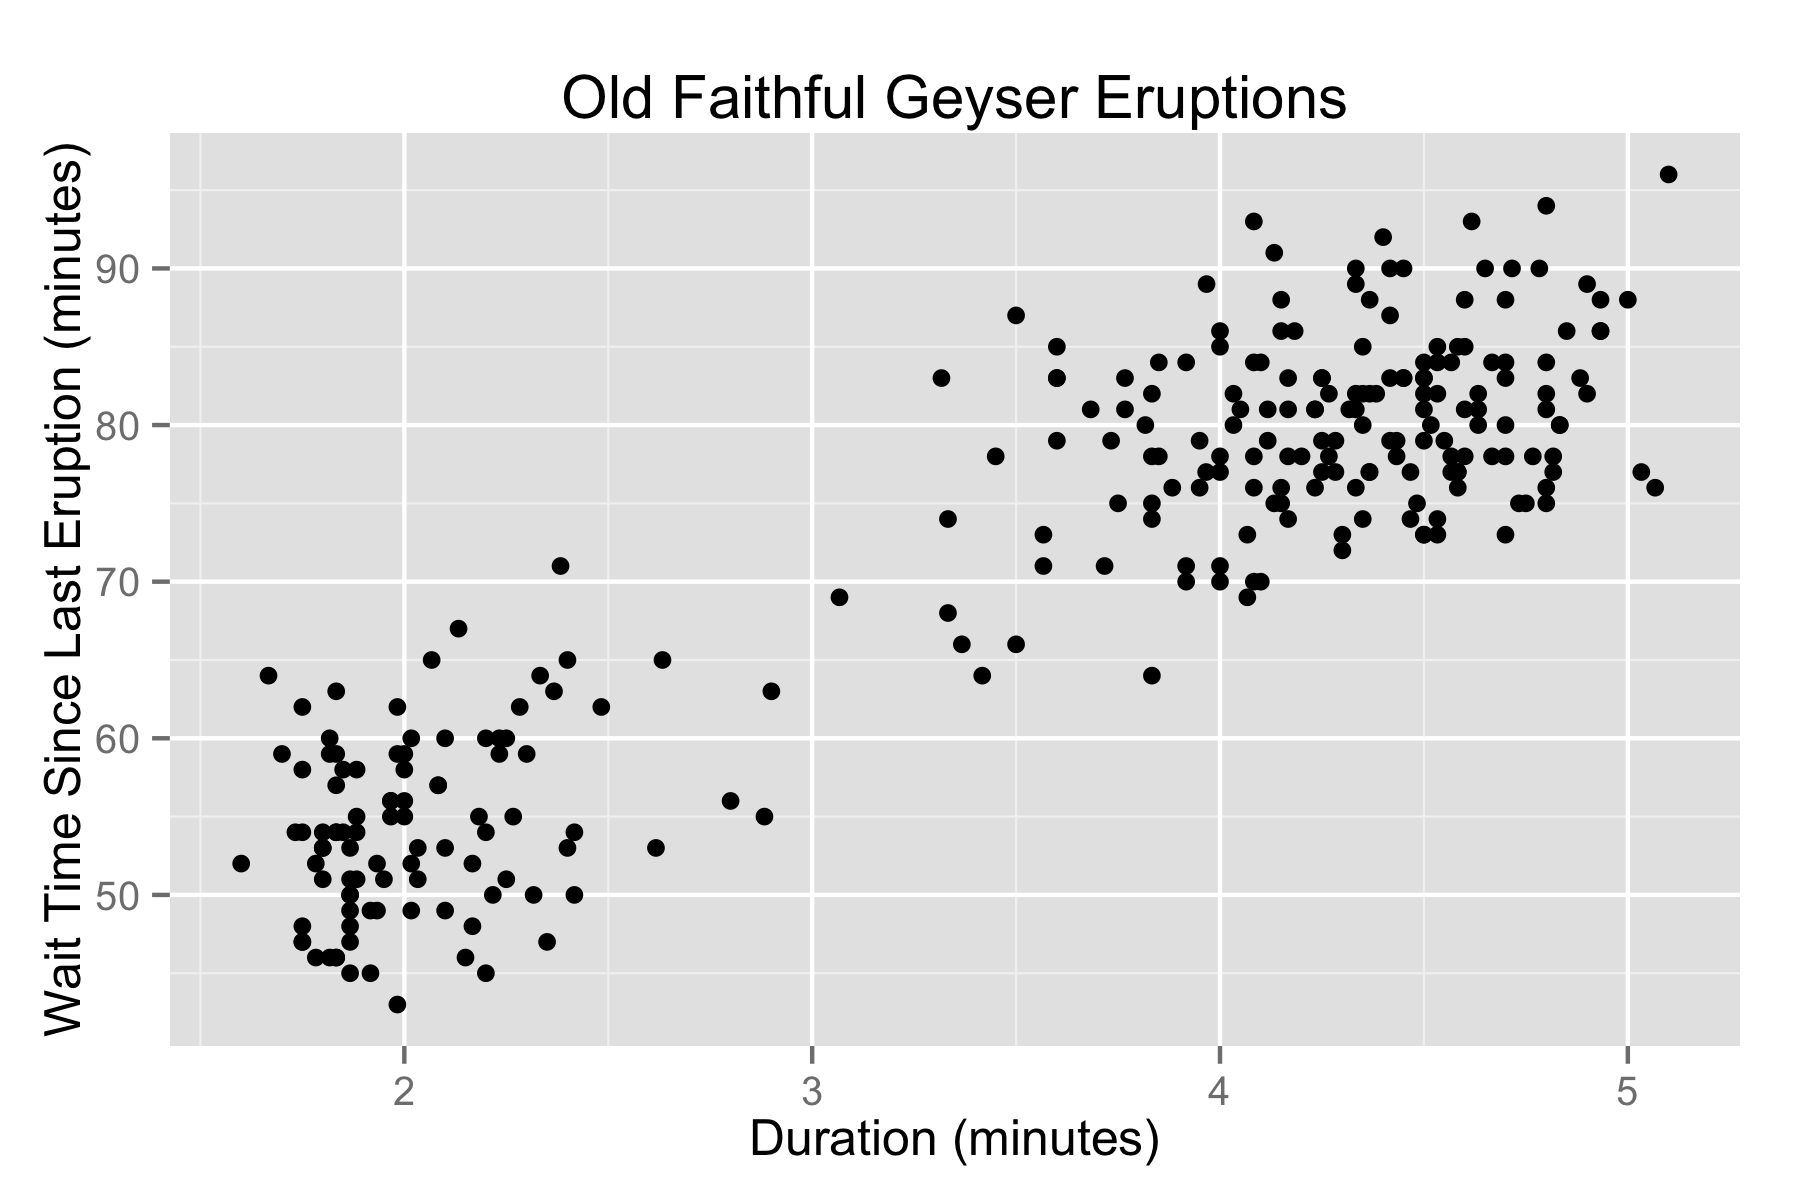
\includegraphics[height=0.6\textheight]{figures/oldfaithful}
\begin{itemize}
\item Looks like two clusters.
\item How to find these clusters algorithmically?
\end{itemize}
\note[item]{Let's consider a simple example. The old faithful geyser in Yellowstone has very predictable eruptions. It roughly erupts every 55 or 80 minutes. We can visualize this for 2D data, but how do we find these clusters more generally?}
\note[item]{One popular and simple algorithm is $k$-means. Let's go through the algorithm through this example.}
\end{frame}

\begin{frame}{$k$-Means: By Example}

\begin{itemize}
\item Standardize the data.
\item Choose two cluster centers.
\end{itemize}
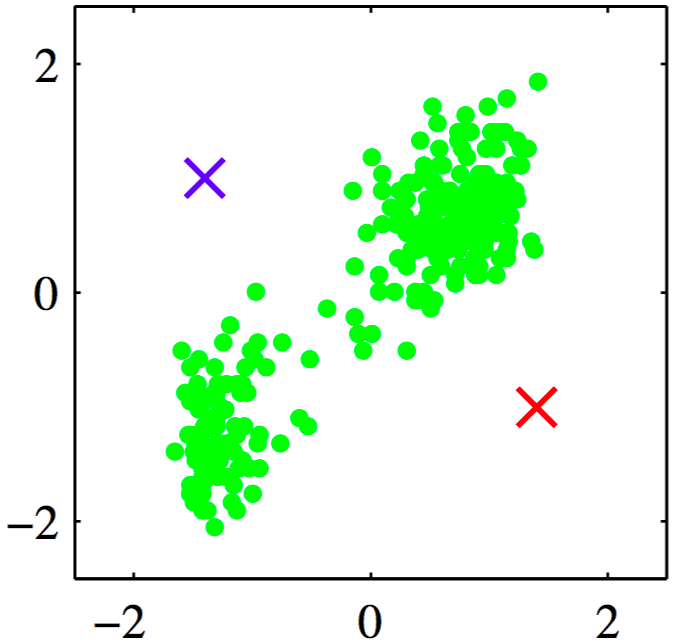
\includegraphics[height=0.55\textheight]{{figures/faithful-9.1a}}

\let\thefootnote\relax\footnotetext{\tiny{From Bishop's \emph{Pattern recognition and machine learning}, Figure 9.1(a).}}
\note[item]{We first standardize the data and choose two points randomly. They will be the cluster center.}
\end{frame}

\begin{frame}{$k$-means: by example}

\begin{itemize}
\item Assign each point to closest center.
\end{itemize}
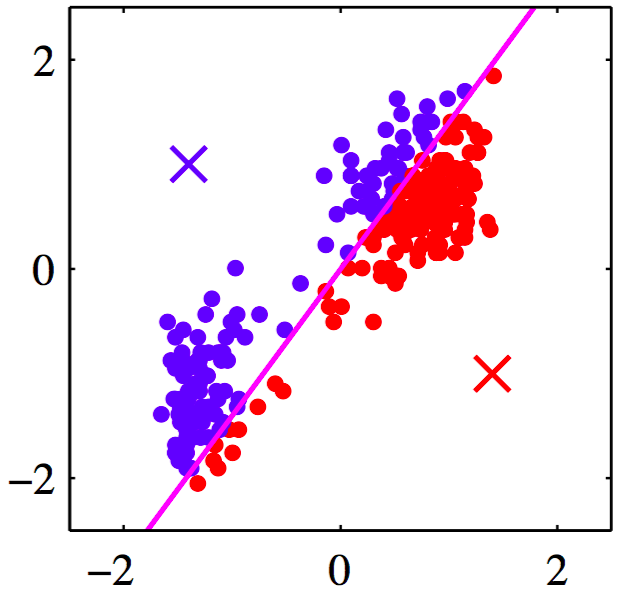
\includegraphics[height=0.55\textheight]{{figures/faithful-9.1b}}

\let\thefootnote\relax\footnotetext{\tiny{From Bishop's \emph{Pattern recognition and machine learning}, Figure 9.1(b).}}
\end{frame}
%
\begin{frame}{$k$-means: by example}

\begin{itemize}
\item Compute new cluster centers.
\end{itemize}
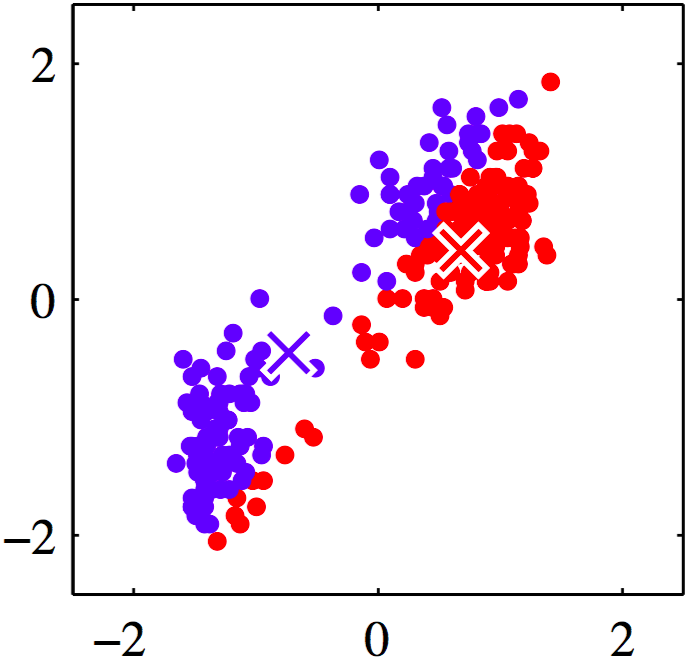
\includegraphics[height=0.55\textheight]{{figures/faithful-9.1c}}

\let\thefootnote\relax\footnotetext{\tiny{From Bishop's \emph{Pattern recognition and machine learning}, Figure 9.1(c).}}
\end{frame}
%
\begin{frame}{$k$-means: by example}

\begin{itemize}
\item Assign points to closest center.
\end{itemize}
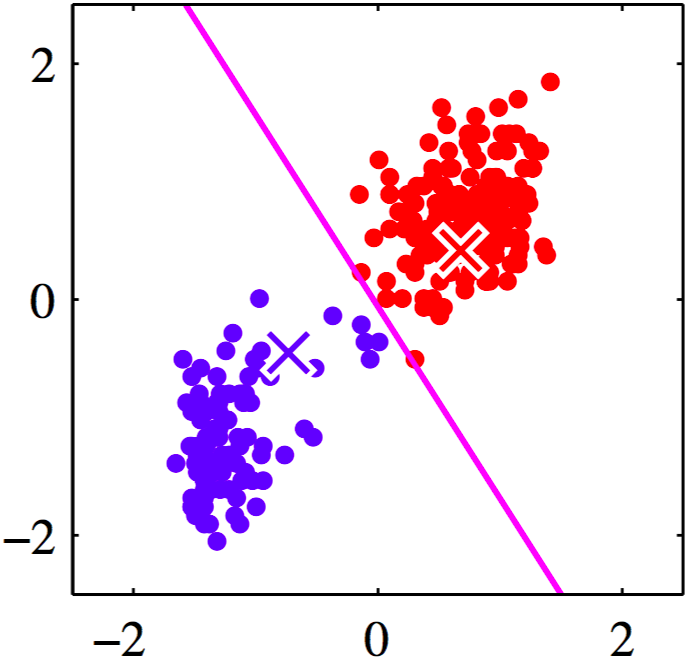
\includegraphics[height=0.55\textheight]{{figures/faithful-9.1d}}

\let\thefootnote\relax\footnotetext{\tiny{From Bishop's \emph{Pattern recognition and machine learning}, Figure 9.1(d).}}
\end{frame}
%
\begin{frame}{$k$-means: by example}

\begin{itemize}
\item Compute cluster centers.
\end{itemize}
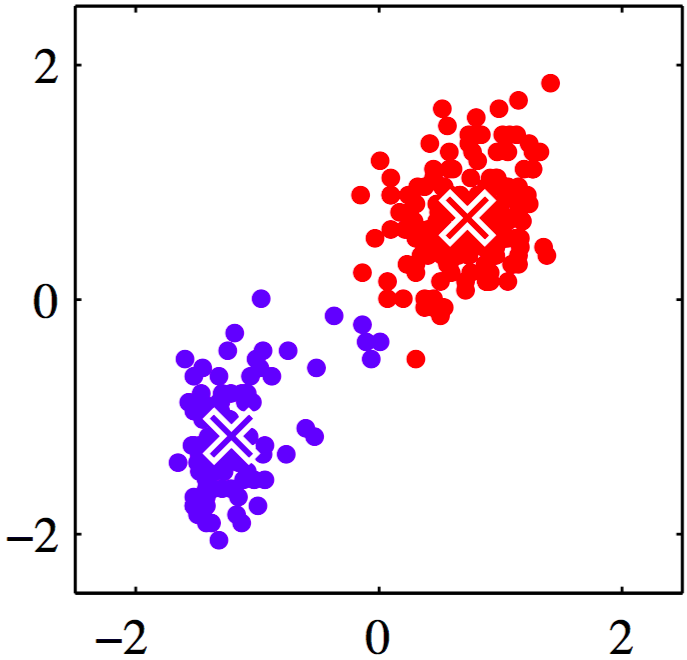
\includegraphics[height=0.55\textheight]{{figures/faithful-9.1e}}

\let\thefootnote\relax\footnotetext{\tiny{From Bishop's \emph{Pattern recognition and machine learning}, Figure 9.1(e).}}
\end{frame}
%
\begin{frame}{$k$-means: by example}

\begin{itemize}
\item Iterate until convergence.
\end{itemize}
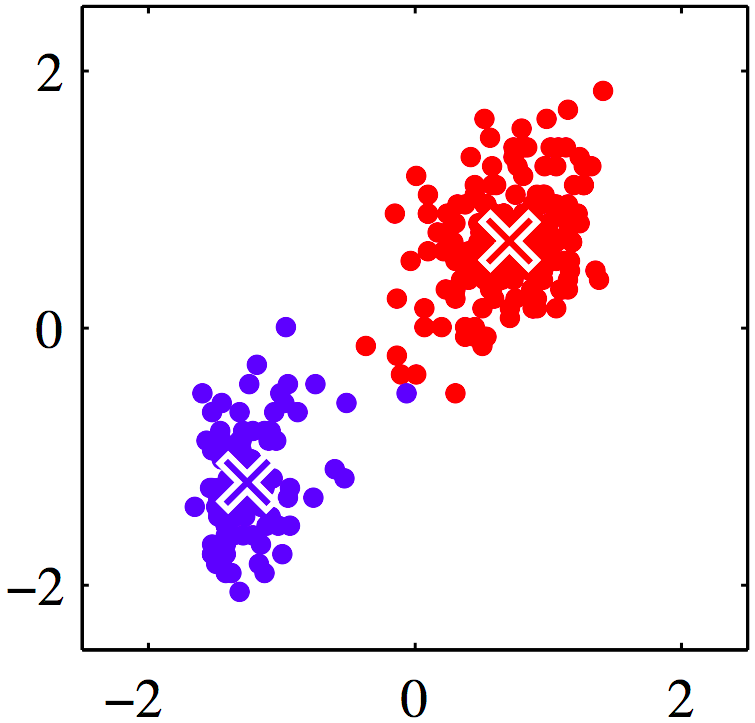
\includegraphics[height=0.55\textheight]{{figures/faithful-9.1i}}

\let\thefootnote\relax\footnotetext{\tiny{From Bishop's \emph{Pattern recognition and machine learning}, Figure 9.1(i).}}
\note[item]{When do we achieve convergence? The cluster assignments no longer change.}
\note[item]{Does it always converge? Yes, more on this later.}
\note[item]{Does it always converge to good clusters? Not necessarily.}
\end{frame}

\begin{frame}{Suboptimal Local Minimum}

\begin{itemize}
\item The clustering for $k=3$ below is a local minimum, but suboptimal:
\end{itemize}
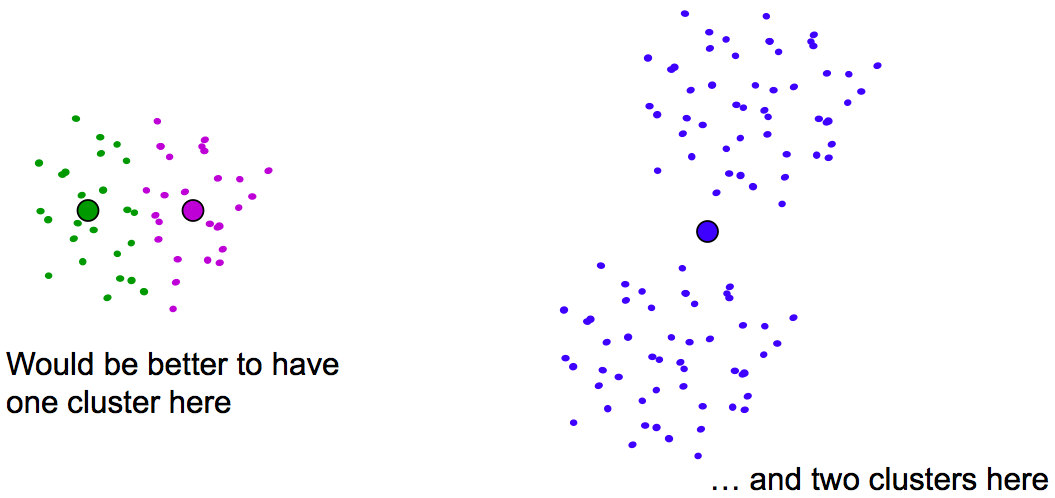
\includegraphics[width=0.8\textwidth]{figures/k-means-local-optimum}\let\thefootnote\relax\footnotetext{\tiny{From Sontag's DS-GA 1003, 2014, Lecture 8.}}
\note[item]{In this example, we have 3 clusters. But $k$-means found different cluster assignments than what we would do. It's a stationary point even though we can find ``better'' clusters.}
\note[item]{How do we define ``good'' clusters? Let's formalize $k$-means with an objective function.}
\end{frame}
%

\begin{frame}{Formalize $k$-Means}
\begin{itemize}[<+->]
\item Dataset $\cd=\left\{ x_{1},\ldots,x_{n}\right\} \subset\cx$ where $\sX = \reals^d$.

\item Goal: Partition data $\cd$ into $k$ disjoint sets $C_{1},\ldots,C_{k}$.
\item Let $c_i \in \pc{1, \ldots, k}$ be the cluster assignment of $x_i$.

\item The \textbf{centroid} of $C_{i}$ is defined to be
\begin{align}
\mu_{i}=\argmin_{\mu\in\cx}\sum_{x\in C_{i}}\|x - \mu\|^{2}.
&& \text{mean of $C_i$}
\end{align}

\item The $k$-means objective is to minimize the distance between each example and its cluster centroid:
\begin{align}
J(c, \mu) = \sum_{i=1}^n \| x_i - \mu_{c_i} \|^2 .
\end{align}
\end{itemize}
\note[item]{Define the centroid as the point that minimizes its distance to all other points in the cluster. In $\reals^d$,  the distance is Euclidean distance. If you solve this optimization problem, the centroid is the cluster mean.}
\end{frame}

%
\begin{frame}{$k$-Means: Algorithm}
\begin{enumerate}[<+->]
\item Initialize: Randomly choose initial centroids $\mu_{1},\ldots,\mu_{k} \in \reals^d$.

\item Repeat until convergence (i.e. $c_i$ doesn't change anymore):

\begin{enumerate}
\item For all $i$, set
\begin{align}
c_i \leftarrow \argmin_j \| x_i - \mu_j \|^2 .
&& \onslide<6->{\text{Minimize $J$ w.r.t. $c$ while fixing $\mu$}}
\end{align}

\item For all $j$, set 
\begin{align}
\mu_{j} \leftarrow \frac{1}{|C_j|}\sum_{x\in C_j} x .
&& \onslide<7->{\text{Minimze $J$ w.r.t. $\mu$ while fixing $c$.}}
\end{align}
\end{enumerate}
\end{enumerate}
\begin{itemize}
\item<5-> Recall the objective: $J(c, \mu) = \sum_{i=1}^n \| x_i - \mu_{c_i} \|^2$.
%\item<8-> $k$-means is coordinate descent on $J$.
\end{itemize}
\note[item]{Repeat two steps iteratively until convergence. 1) Assign points to their nearest cluster, where the distance is measured by the Euclidean distance between the point and the cluster centroid. 2) Update the cluster centroid given the assignments in the first step.}
\note[item]{Is this algorithm minimizing the objective?}
\note[item]{If we optimize the objective wrt each var while fixing other vars, what is it called?}
\end{frame}
%
\begin{frame}{Avoid bad local minima}
\begin{simpleblock}
{$k$-means converges to a local minimum.}
\begin{itemize}
%\item $k$-means is coordinate descent on $J$, thus $J$ will monotonically decrease.
\item $J$ is non-convex, thus no guarantee to converging to the global minimum.
\end{itemize}
\end{simpleblock}


\begin{simpleblock}
{Avoid getting stuck with bad local minima:}

\begin{itemize}[<+->]
\item Re-run with random initial centroids.
\item \textbf{$k$-means++}: choose initial centroids that spread over all data points.
\begin{itemize}[<+->] 
\item Randomly choose the first centroid from the data points $\cd$.
\item Sequentially choose subsequent centroids from points that are farther away from current centroids:
\begin{itemize}[<+->]
\item Compute distance between each $x_{i}$ and the closest already chosen
centroids.
\item Randomly choose next centroid with probability proportional to the
computed distance squared.
\end{itemize}
\end{itemize}
\end{itemize}
\end{simpleblock}

\note[item]{It can be shown that $k$-means++ converges to a solution not much worse than the optimal solution. Specifically, $\mathbb{E}\pb{J_{k\text{-means}++}} \le O(\log k) J^*$.}
\end{frame}

\begin{frame}
{Summary}
\begin{simpleblock}
{We've seen}
\begin{itemize}
\item Clustering---an unsupervised learning problem that aims to discover group assignments.
\item $k$-means:
\begin{itemize}
\item Algorithm: alternating between assigning points to clusters and computing cluster centroids.
\item Objective: minmizing some loss function by cooridinate descent.
\item Converge to a local minimum.
\end{itemize}
\end{itemize}
\end{simpleblock}

\onslide<2->{
\begin{simpleblock}
{Next, probabilistic model of clustering.}
\begin{itemize}
\item A generative model of $x$.
\item Maximum likelihood estimation.
\end{itemize}
\end{simpleblock}
}
\note[item]{At the beginning, we mentioned that unsupervised learning is often formulated as density estimation. But the $k$-means algorithm is not probabilistic. So next let's consider a probabilistic model of clustering and we will show that $k$-means is a special case of this approach.}
\end{frame}


\end{document}
